\setchapterabstract{本讲回顾了 Transformer 及其 modern variants,重点讨论 normalization (Pre-norm, RMSNorm)、activation functions (ReLU, GeLU, SwiGLU)、position embeddings (absolute, relative, RoPE),并总结 hyperparameter choices、training stability tricks 以及 attention variants (MQA, GQA, sparse attention)。}

\vspace{-10cm}
\chapter{Architectures variations \& Hyperparameters \& Stability tricks}

\vspace{-2cm}

%%%%%%INSERT TOC BELOW 1ST SECTION%%%%%%%%%%%%

{\chaptoc\noindent\begin{minipage}[inner sep=0,outer sep=0]{0.9\linewidth}\section{The Original Transformer \& Modern Variants}\end{minipage}}
\\

\subsection{Review of the Original Transformer}

\begin{figure}[htbp]
  \centering
  \begin{minipage}{0.45\linewidth}
    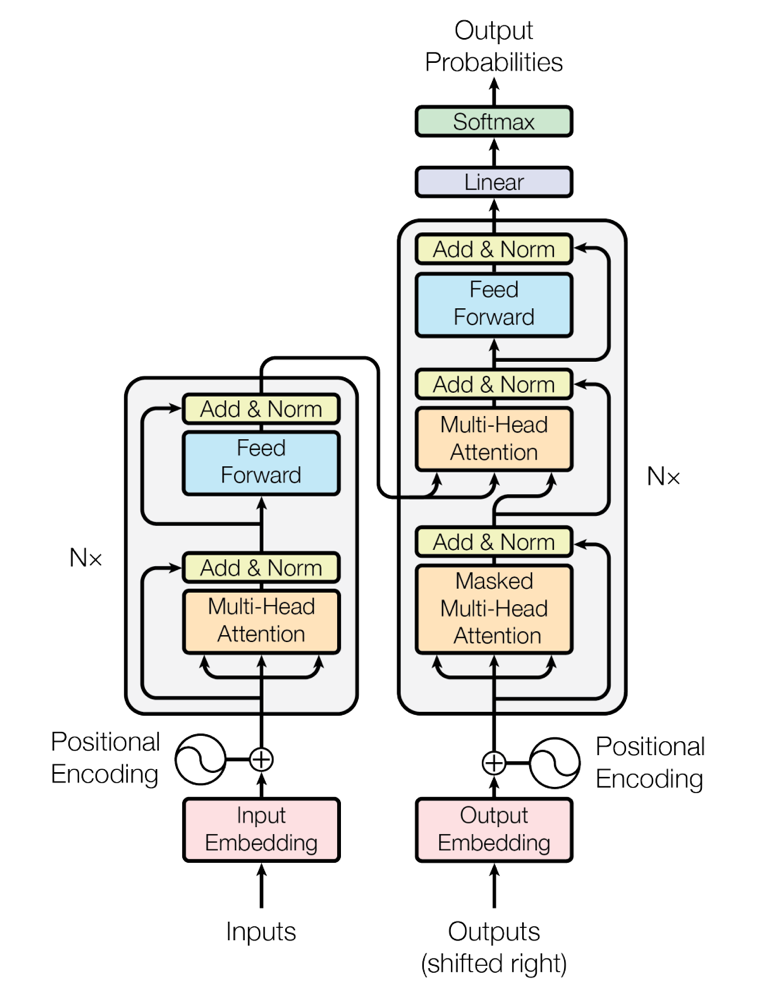
\includegraphics[width=\linewidth]{figs/lec3/lec3.01.png}
    \caption{The original Transformer architecture}
  \end{minipage}
  \hfill
  \begin{minipage}{0.5\linewidth}
    \small
    在Original Transformer Architecture中,我们在选择以下方式来构建Architecture
    \begin{itemize}
    \item \textbf{Norm Type}: Post-norm, LayerNorm
    \item \textbf{FFN Type}: ReLU \\
        \[
        \text{FFN}(z_i) = \text{ReLU}(z_i W_1 + b_1) W_2 + b_2
        \]
    \item \textbf{Position Embedding}: sines and cosines \\
    \begin{align*}
     &\mathrm{PE}(pos,\, 2i)   = \sin \Bigl( pos \,/\, 10000^{\,2i / d_{\mathit{model}}} \Bigr)\\
     &\mathrm{PE}(pos,\, 2i+1) = \cos \Bigl( pos \,/\, 10000^{\,2i / d_{\mathit{model}}} \Bigr)
    \end{align*}
    
    \end{itemize}
    而这些有许多变体,接下来我们会逐一介绍:
    \begin{itemize}
        \item Pre-norm vs. Post-norm
        \item LayerNorm vs. RMSNorm
        \item ReLU, GeLU, *GLU, SwiGLU
        \item Serial vs. Parallel layers
        \item Relative Position Embeddings vs. Absolute Position Embeddings
    \end{itemize}
  \end{minipage}
\end{figure}


\MarginImageWithNote
  {figs/lec3/lec3.02.png}
  {\captionof{figure}{Modern Models' Architecture}}


\clearpage
\subsection{Normalization Variants}
\subsubsection{Pre-norm vs. Post-norm}~{}
\\
\MarginImageWithNote
  {figs/lec3/lec3.02.png}
  {\captionof{figure}{Pre-norm vs. Post-norm in Transformer}}


\begin{figure}[htbp]
  \centering
  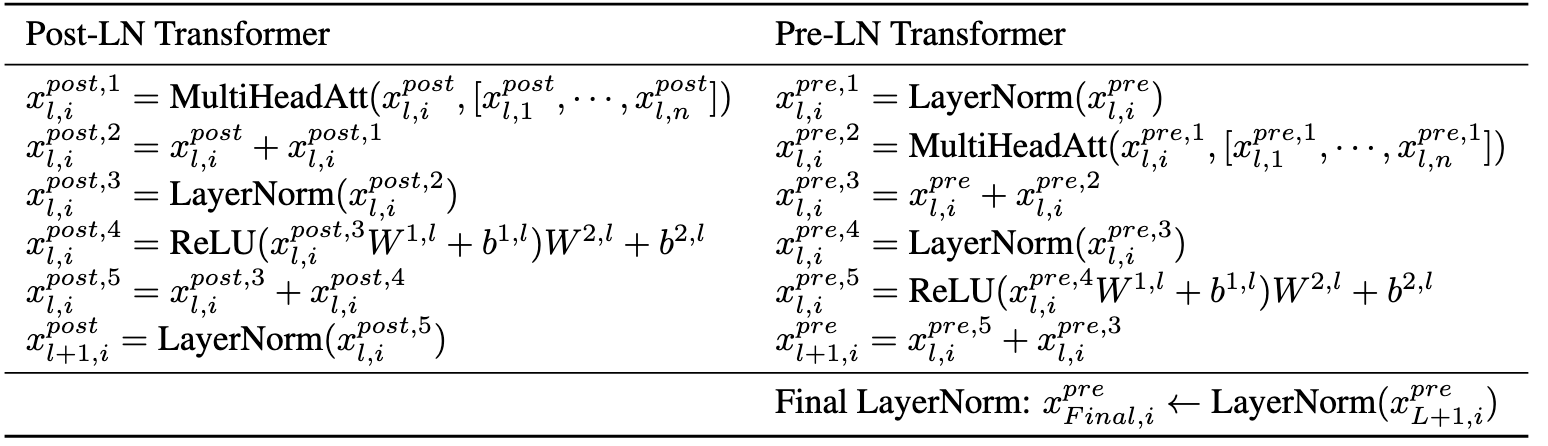
\includegraphics[width=1\linewidth]{figs/lec3/lec3.04.png}
  \caption{}
  \label{fig:}
\end{figure}





\subsubsection{Double Norm}

\subsubsection{LayerNorm vs. RMSNorm}





\subsection{Activation Variants}

\subsection{Serial vs. Parallel layers}

\subsection{RoPE: Rotary Position Embeddings}




























\clearpage
{\chaptoc\noindent\begin{minipage}[inner sep=0,outer sep=0]{0.9\linewidth}\section{Hyperparameters}\end{minipage}}
\\


\subsection{Feedforward Dimension Ratio}

\subsection{Head Dimension and Model Dimension}

\subsection{Aspect Ratio}

\subsection{Vocabulary Size}

\subsection{Regularization}



\clearpage
{\chaptoc\noindent\begin{minipage}[inner sep=0,outer sep=0]{0.9\linewidth}\section{Stability tricks}\end{minipage}}
\\

\subsection{Output Softmax Stability}

\subsection{Attention Softmax Stability}

\subsection{Logit Soft-Capping}



\clearpage
{\chaptoc\noindent\begin{minipage}[inner sep=0,outer sep=0]{0.9\linewidth}\section{Attention Heads}\end{minipage}}
\\

\subsection{Grouped-Query Attention \& Multi-Query Attention}

\subsection{Sparse/Sliding Window Attention}

\subsection{Hybrid Approaches}

% 图 1:OPT FLOPs 构成
% \MarginImageWithNote
%   {figs/}
%   {\captionof{figure}{}}
%   {
%   }

% \begin{figure}[htbp]
%   \centering
%   \includegraphics[width=1\linewidth]{figs/lec1/.png}
%   \caption{}
%   \label{fig:}
% \end{figure}


